
Con este experimento se pretende demostrar las diferencias  entre la medición de voltaje en alterna, entre un voltímetro tradicional y otro con \textit{TrueRMS}. 

Las diferencias de funcionamiento entre estos fueron establecidas en la sub-sección \ref{sec:VoltCA} del Marco Teórico. 

Se compararon dos señales, una triangular y una cuadrada, ambas de 50 Hz y 5 $V_{pp}$. Estas fueron generadas por el generador de ondas de la marca GW-INSTEK, modelo GFG-3015.

El circuito utilizado para la medición es el siguiente (figura \ref{fig:exp3med}):

\begin{figure}[H]
    \centering
    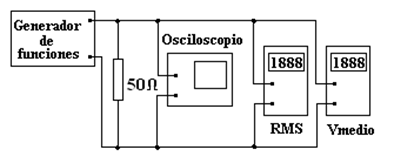
\includegraphics[width=0.6\linewidth]{Imagenes/exp3med.png}
    \caption{Circuito Experimento 3}
    \label{fig:exp3med}
\end{figure}

Se tomó como resistencia de carga de 50 $\Omega$, la resistencia interna a la salida del generador.


\unsubsubsection{Cálculos}

Antes de realizar las mediciones, se realizaron los cálculos con los valores y forma de onda propuestas para saber más o menos cuanto debíamos medir en cada caso.

Para la onda cuadrada (con centro en 0 y $V_p = 2.5 V$): 

\begin{equation}
    V_{ef_C} = V_p
    \hspace{5mm}\Longrightarrow\hspace{5mm}
    V_{ef_C} = 2.5~V
\end{equation}

Y para la onda triangular (con centro en 0 y $V_p = 2.5 V$): 

\begin{equation}
    V_{ef_T} = \cfrac{V_p}{\sqrt{3}}
    \hspace{5mm}\Longrightarrow\hspace{5mm}
    V_{ef_T} = \cfrac{2.5~V}{\sqrt{3}} = 1.443~V
\end{equation}

\unsubsubsection{Mediciones}

A continuación, se presentan las mediciones en una tabla y junto a ellas un porcentaje de error. Este porcentaje corresponde al valor porcentual de la diferencia entre las mediciones, con respecto a la medición con \textit{TrueRMS}, que se supone es la real y correcta. 

\begin{table}[H]
    \centering
    \begin{tabular}{|c|c|c|c|c|}
    \hline
        \multicolumn{2}{|c|}{Generador} & RMS [V] & $V_{medio}$ [V] & e\% \\
    \hline
        50 Hz & Cuadrada & 2.528 & 2.76 & 9.177\% \\
    \cline{2-5}
        5 $V_{pp}$ & Triangular & 1.453 & 1.35 & 7.088\% \\
    \hline
        \end{tabular}
        \def\tablename{Tabla} 
        \caption{Tabla de mediciones con porcentaje de error entre ellas}
        \label{tab:RMSvsVm}
\end{table}

Como era de esperarse, las mediciones con el multimetro \textit{TrueRMS} fueron bastante acertadas. Coinciden casi totalmente con los valores calculados anteriormente.

En cuanto al porcentaje de error entre mediciones, este parece ser bastante bajo, pero suficiente para ver que le falta el factor de corrección. A pesar de su poca diferencia, no hay que dejarse engañar, ya que en estos dos casos, las señales son centradas en cero y con formas similares a una sinusoidal (para la que esta diseñado). Este porcentaje de error probablemente se incrementaría notablemente si la señal medida fuera por ejemplo una onda de diente de sierra o algún otro tipo de onda un poco menos simétrica.

\begin{figure}[H]
    \begin{subfigure}{0.45\textwidth}
        \centering
        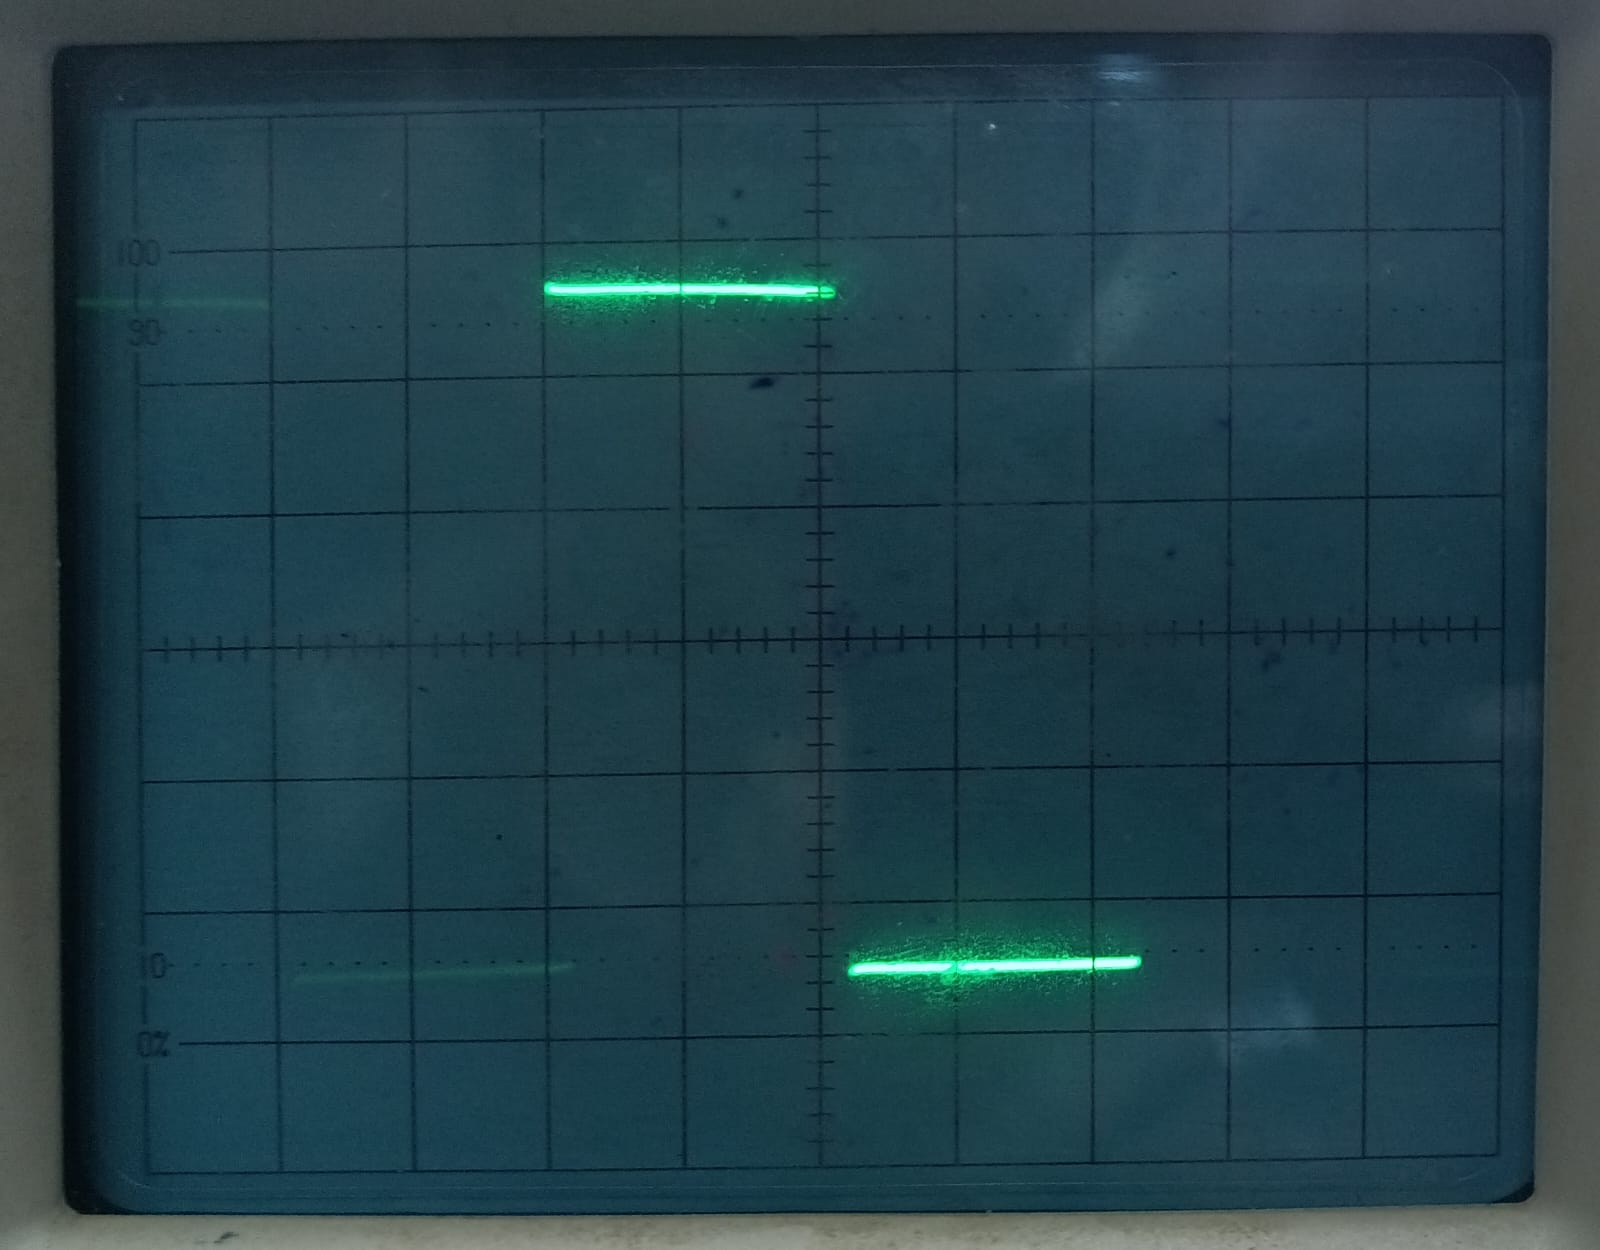
\includegraphics[width=1\linewidth]{Imagenes/Cuad3.jpeg}
        \caption{Señal Cuadrada}
        \label{fig:desfExp1}
    \end{subfigure}
    \hspace*{\fill}
    \begin{subfigure}{0.45\textwidth}
        \centering
        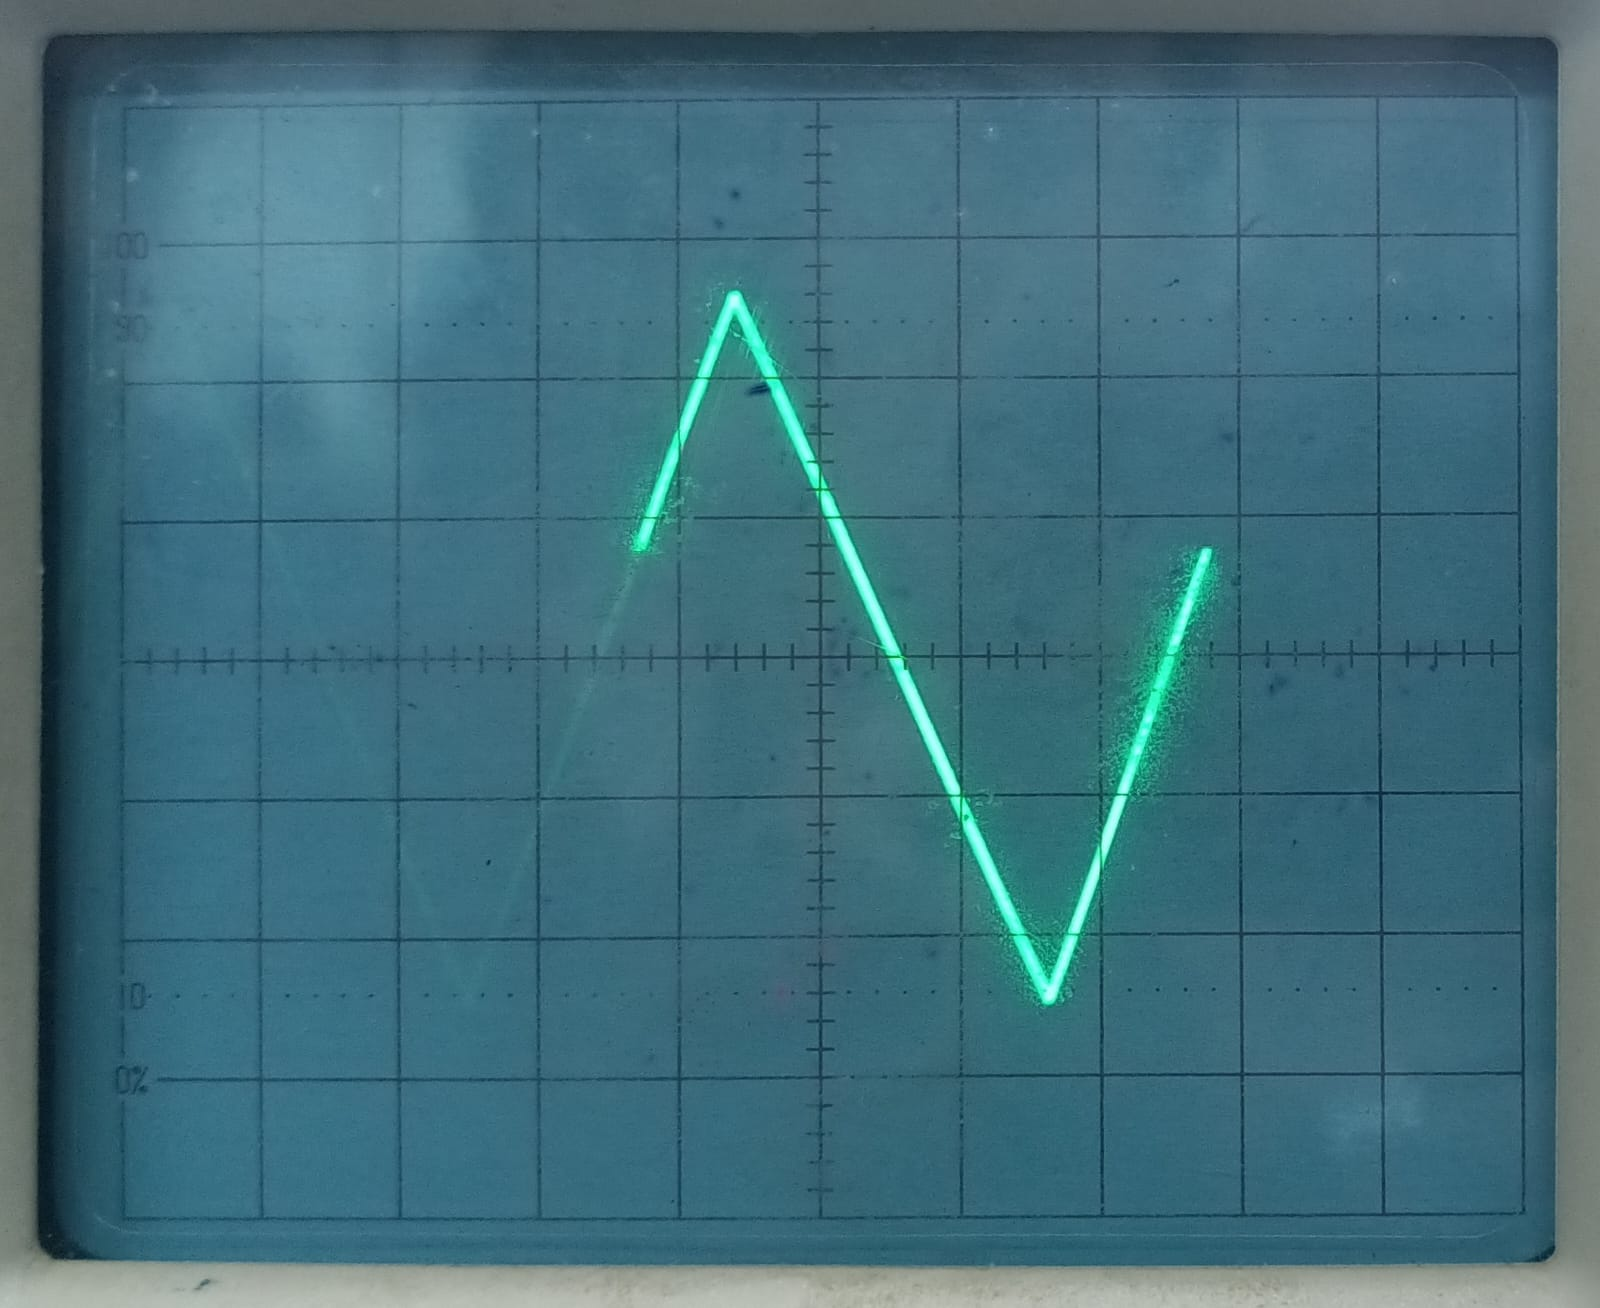
\includegraphics[width=0.96\linewidth]{Imagenes/Triang3.jpeg}
        \caption{Señal Triangular}
        \label{fig:corrFp}
    \end{subfigure}
    \caption{Señales medidas en este experimento}
\end{figure}

Las señales no se llegan a apreciar perfectamente en la figura debido a su baja frecuencia, la cual era menor que la de muestreo de la cámara con la que se tomaron las fotos.

\unsubsubsection{Factor de Corrección}

Por último, en este experimento se pedía calcular un factor de corrección para que al multiplicar la medición de $V_{medio}$, por este, resultara en el valor eficaz real. Esto se calculó para cada caso, mediante la ecuación \ref{eq:kexp3}:  

\begin{equation}
    \label{eq:kexp3}
    V_{RMS}=V_{medio}\cdot\kappa\llrah c\kappa=\frac{V_{RMS}}{V_{medio}}
\end{equation}

Siguiendo este procedimiento, se tiene:

\begin{equation*}
    \kappa_{cuad}= 0.916 
    \hspace{2cm}
    \kappa_{triang}= 1.706
\end{equation*}

Se puede corroborar que este valor es muy similar a los factores de corrección obtenidos de manera analítica en la sección \ref{sec:conc} (Conclusión). Las pequeñas diferencias entre sus valores, podrían deberse a la incertidumbre en la medición de los valores de tensión en este experimento, los cuales terminan afectando la relación entre estos y por tanto el factor de corrección práctico.